\section{Speicher}
\subsection{Schieberegister}
\begin{circuit}[0.35]
    \node[dFf] (dff0) {};
    \node[dFf, right = 7mm of dff0] (dff1) {};
    \node[dFf, right = 7mm of dff1] (dff2) {};
    \node[dFf, right = 7mm of dff2] (dff3) {};

    \node[left = 5mm of dff0.pin 1] (din) {\cirin{D}$_{\text{in}}$};
    \node[below left = 0.5mm and 5mm of dff0] (clk) {\cirin{CLK}};

    \draw[] (din) -- (dff0.pin 1);
    \path[draw] (dff0.pin 6) -- (dff1.pin 1) coordinate[midway] (q0);
    \path[draw] (dff1.pin 6) -- (dff2.pin 1) coordinate[midway] (q1);
    \path[draw] (dff2.pin 6) -- (dff3.pin 1) coordinate[midway] (q2);
    \path[draw] (dff3.pin 6) --++ (right:2mm) coordinate[] (q3);

    \begin{pgfonlayer}{tl1}
        \node[circ, below = 6.2mm of dff0.pin 2] (clkn0) {};
        \node[circ, below = 6.2mm of dff1.pin 2] (clkn1) {};
        \node[circ, below = 6.2mm of dff2.pin 2] (clkn2) {};        
        \node[circ] (qn0) at(q0) {};
        \node[circ] (qn1) at(q1) {};
        \node[circ] (qn2) at(q2) {};
        %\node[circ] (qn3) at(q3) {};
    \end{pgfonlayer}

    \draw[] (clk) -- (clkn0) -- (clkn1) -- (clkn2) -| (dff3.pin 2);
    \draw[] (clkn0) -| (dff0.pin 2);
    \draw[] (clkn1) -| (dff1.pin 2);
    \draw[] (clkn2) -| (dff2.pin 2);

    \path[draw] (q0) --++(90:8mm) node[midway, left] {\cemph[secondaryheader]{LSB}} node[fill = white] {$Q_0$};
    \path[draw] (q1) --++(90:8mm) node[fill = white] {$Q_1$};
    \path[draw] (q2) --++(90:8mm) node[fill = white] {$Q_2$};
    \path[draw] (q3) --++(90:8mm) node[midway, right] {\cemph[secondaryheader]{MSB}} node[fill = white] {$Q_3$};
\end{circuit}
$n$ Flipflops
\begin{itemize}
    \item $n$ Bits gespeichert
    \item $n$ Taktflanken zum einlesen
\end{itemize}
Nachteil: Teuer und Platzintensiv
\subsection{SRAM}
\begin{center}
    \begin{minipage}{0.45\linewidth}
        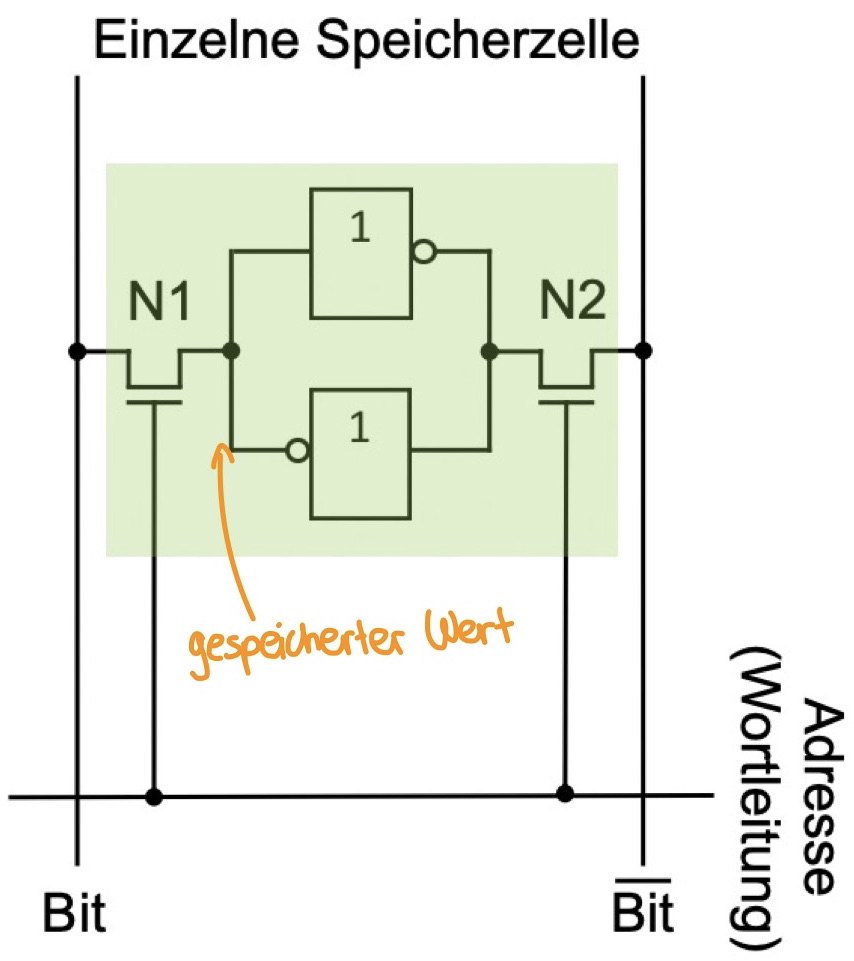
\includegraphics[width = 30mm]{images/sram_store.JPG}
    \end{minipage}
    \hfill
    \begin{minipage}{0.5\linewidth}
        \cemph[black]{Wortleitung}: Anwählen Speicherzelle\\
        \cemph[black]{Bitleitung}: Speicherinhalt lesen oder setzten
        \begin{center}
            \begin{tabular}{c c l}
                Bit & $\overline{\text{Bit}}$ & \\
                1 & 0 & 1 schreiben\\
                0 & 1 & 0 schreiben\\
                1 & 1 & lesen\\
                \multicolumn{3}{l}{Wortleitung bei allen 1.}
            \end{tabular}
        \end{center}
    \end{minipage}
\end{center}
\begin{itemize}
    \item Gespeicherte Wert steht immer auf linker Seite (Bit)
    \item Beim Lesen gibt Bit den Wert zurück; $\overline{\text{Bit}}$ den Invertierten.
    \item Beim Schreiben muss Bit auf den gewünschten Wert und $\overline{\text{Bit}}$ auf den Invertierten gesetzt werden.
\end{itemize}
\paragraph{Lesen}\mbox{}\\
\begin{center}
    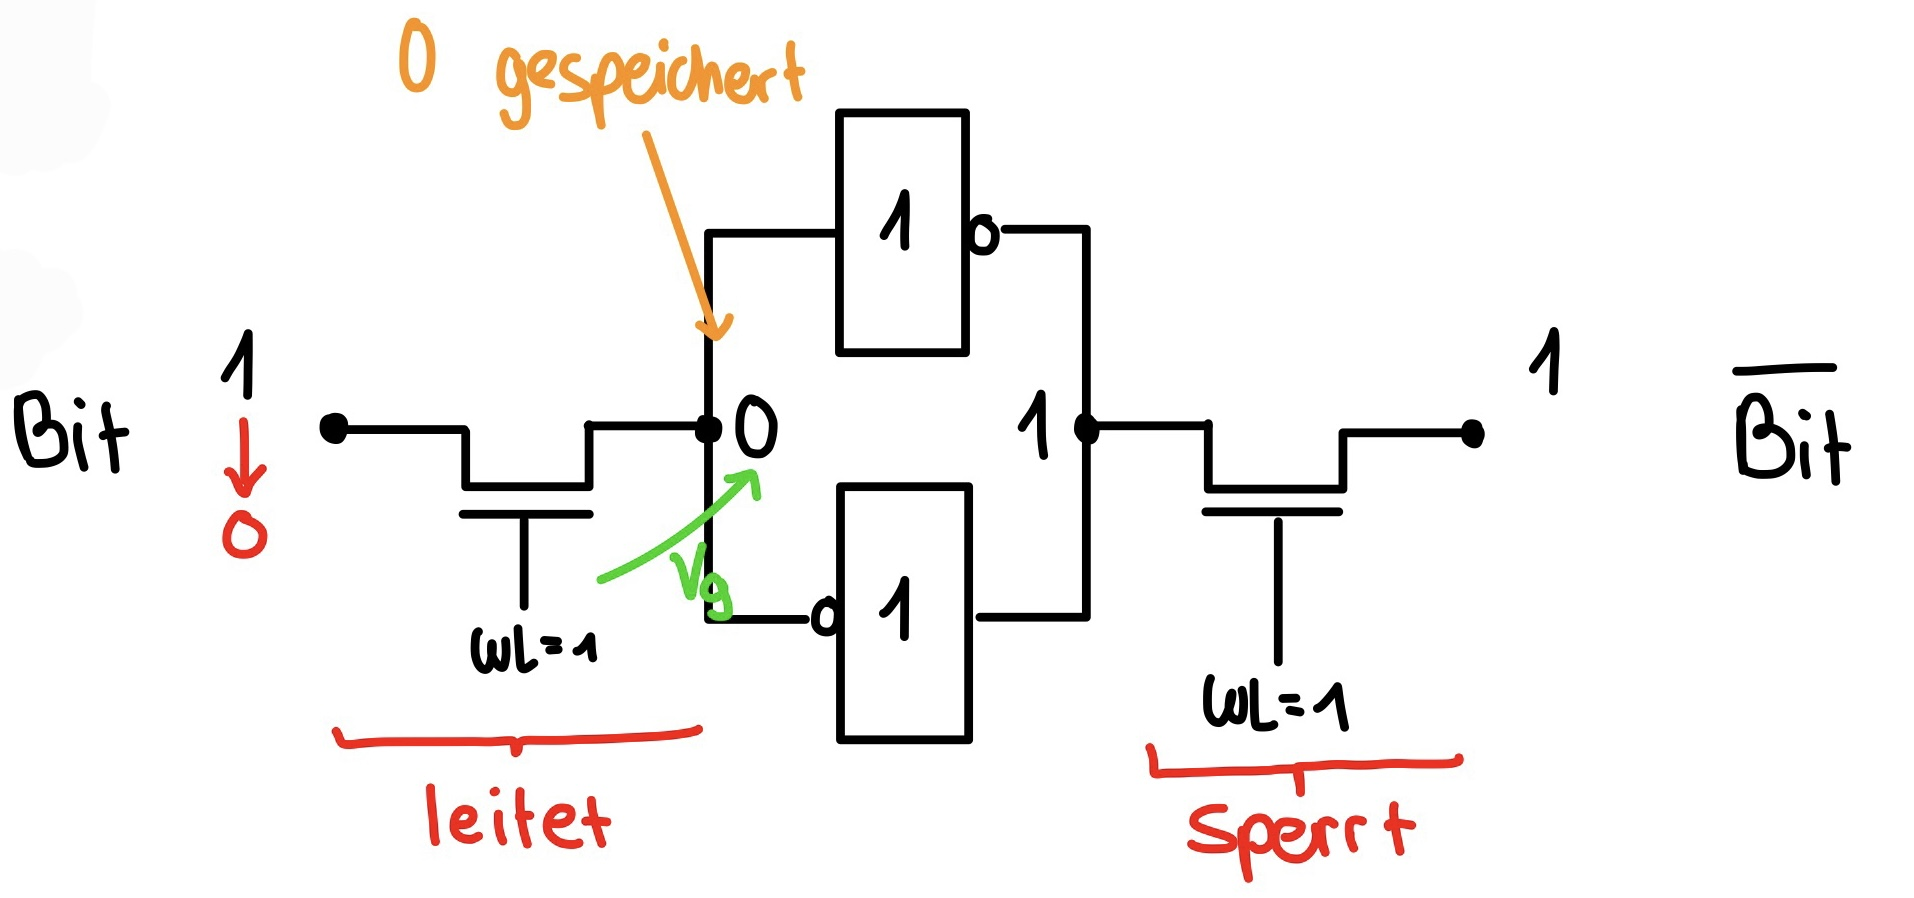
\includegraphics[width = 50mm]{images/sram_read.JPG}
\end{center}
\paragraph{1 Schreiben}\mbox{}\\
\begin{center}
    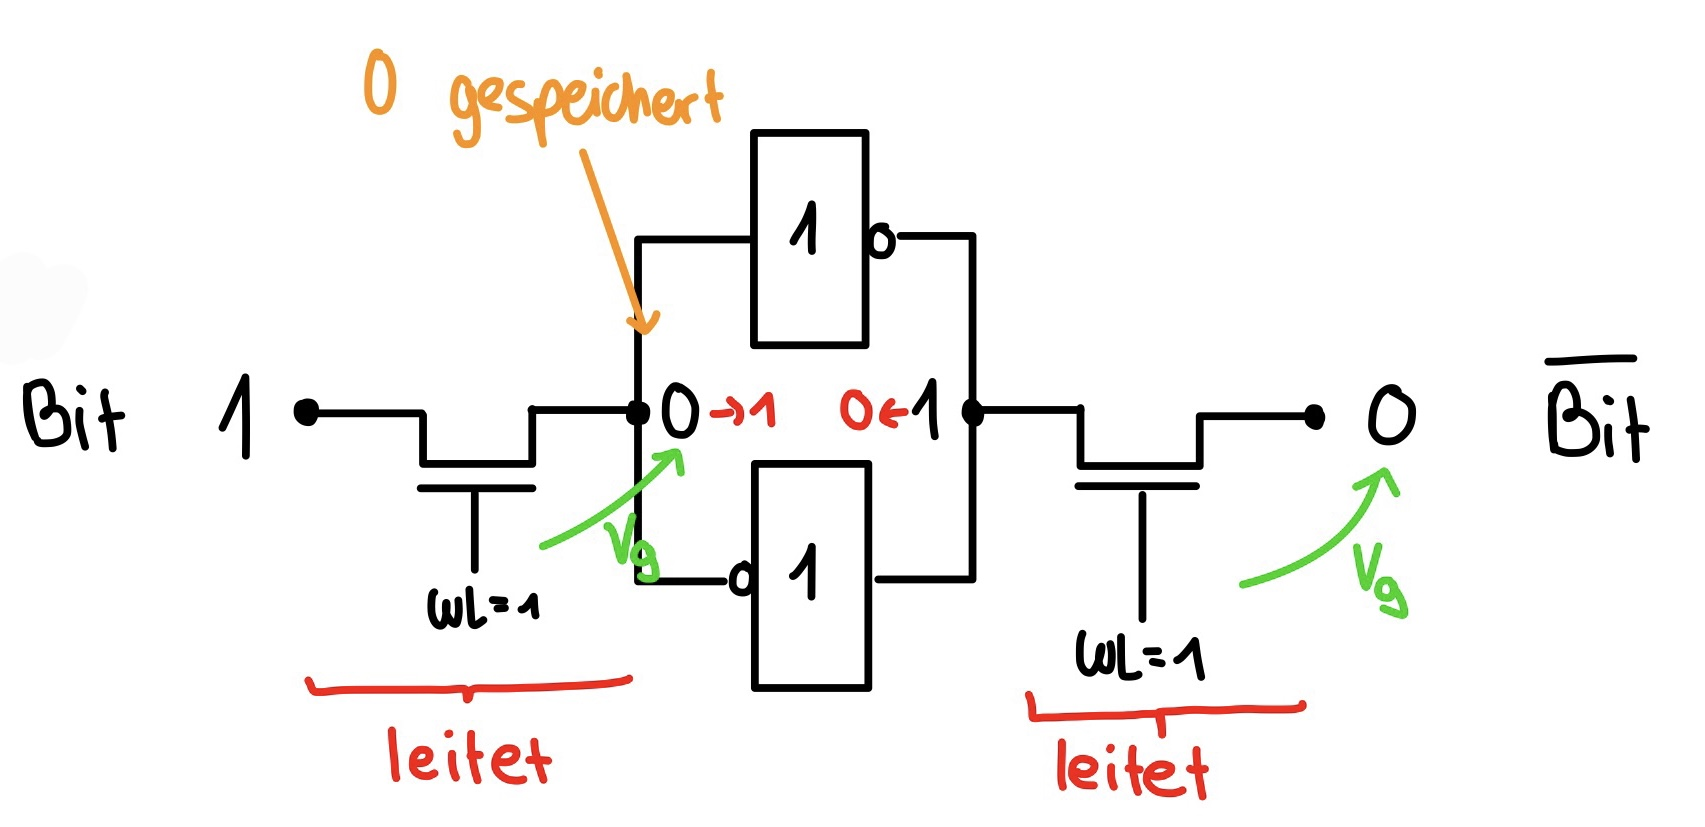
\includegraphics[width =50mm]{images/sram_write.JPG}
\end{center}
\paragraph{0 Schreiben} Gleich wie Schreiben einer 1, aber Bit = 0.

\subsection{DRAM}
\begin{center}
    \begin{minipage}{0.45\linewidth}
        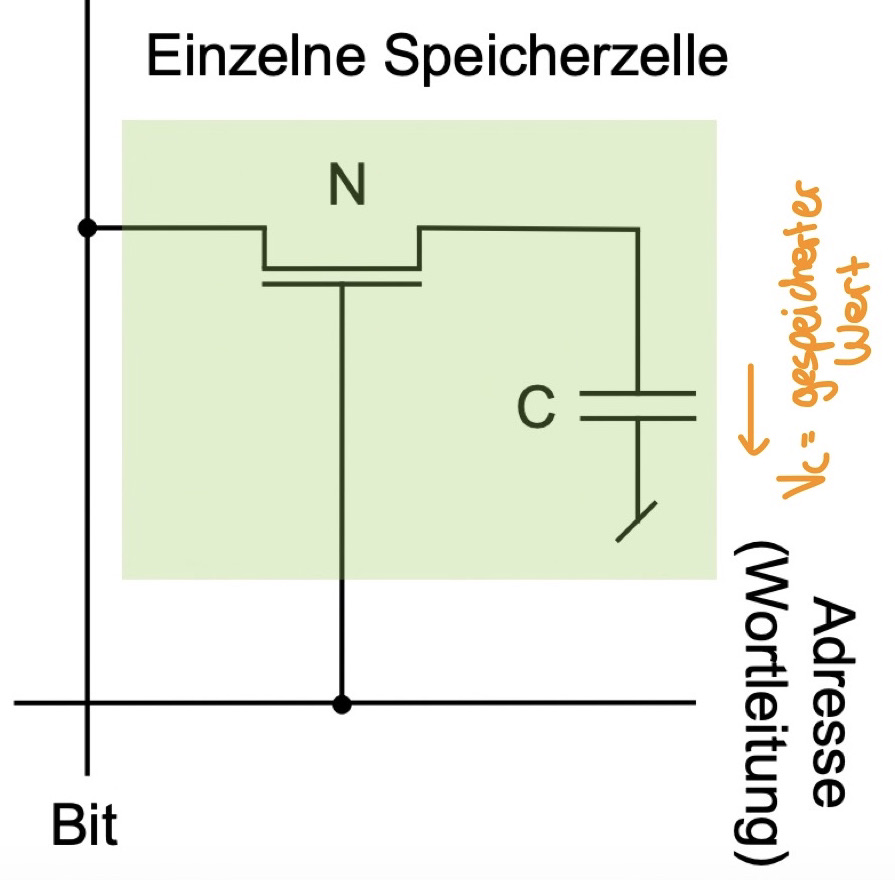
\includegraphics[width = 30mm]{images/dram_store.JPG}
    \end{minipage}
    \hfill
    \begin{minipage}{0.5\linewidth}
        \cemph[black]{Wortleitung}: Anwählen Speicherzelle\\
        \cemph[black]{Bitleitung}: Speicherinhalt lesen oder setzten\\
        \cemph[black]{Schreiben}: Bitleitung wird auf gewünschten Wert gesetzt $\rightarrow$ Kondensator: lädt, entlädt oder bleibt gleich.\\
        \cemph[black]{Lesen}: Parasitäre Kapazität wird ausgenutzt, um aus Veränderung von $V_{\text{out}}$ gespeicherten Wert zu ermitteln.
    \end{minipage}
\end{center}

\subsection{ROM}
Read-Only-Memory wird zur Herstellungszeit als 0 oder 1 programmiert.
\begin{center}
    \begin{minipage}{0.45\linewidth}
        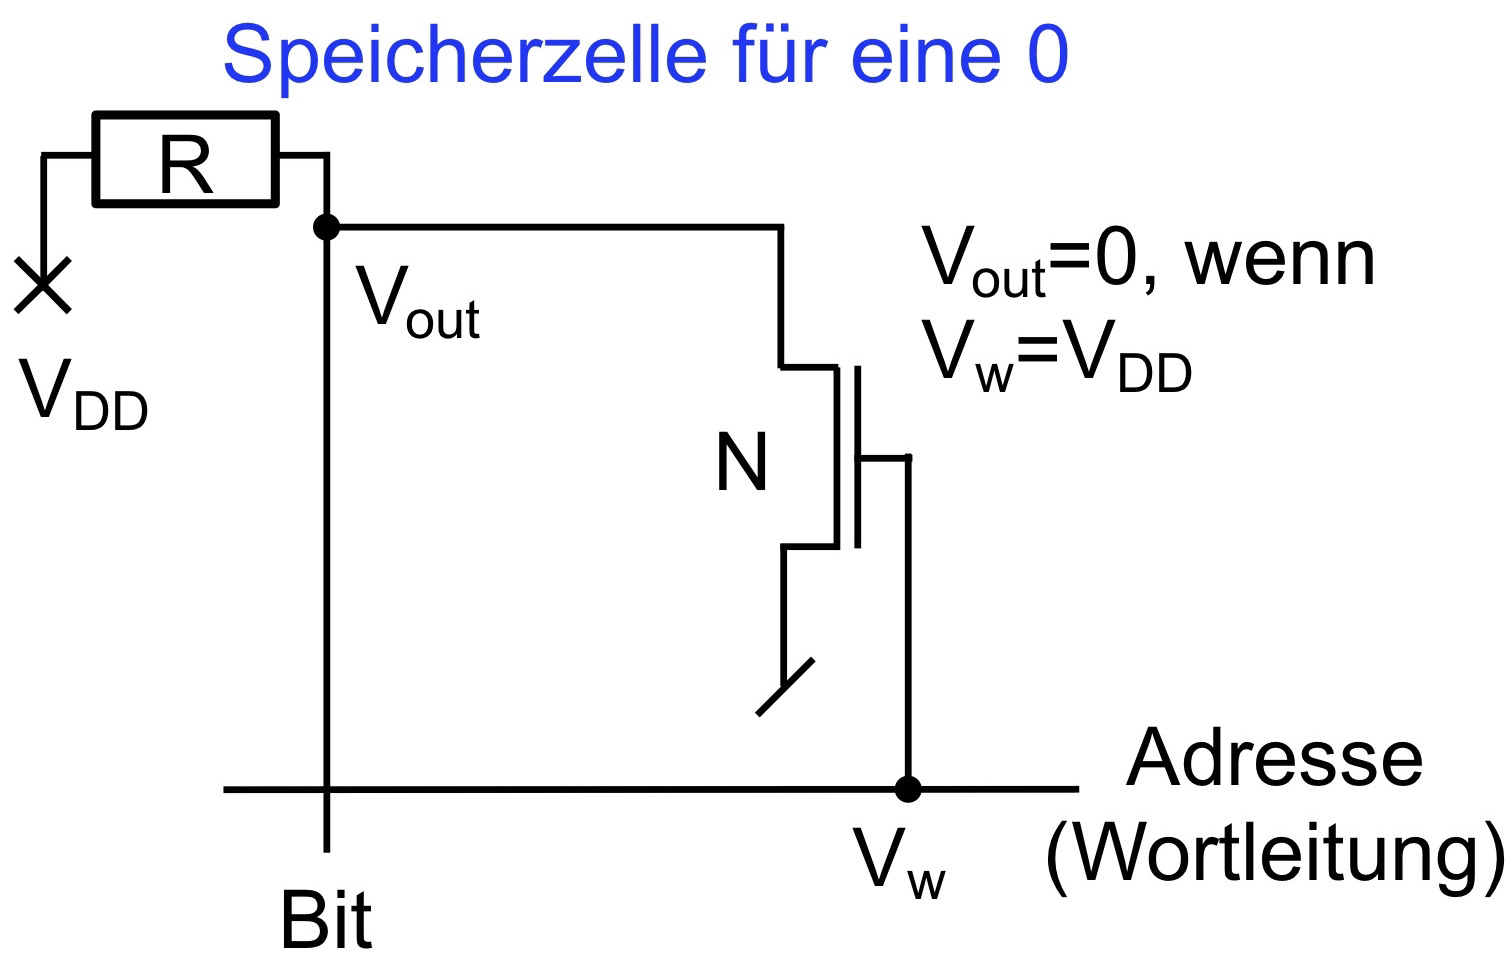
\includegraphics[width = 30mm]{images/rom_0.JPG}
    \end{minipage}
    \hfill
    \begin{minipage}{0.45\linewidth}
        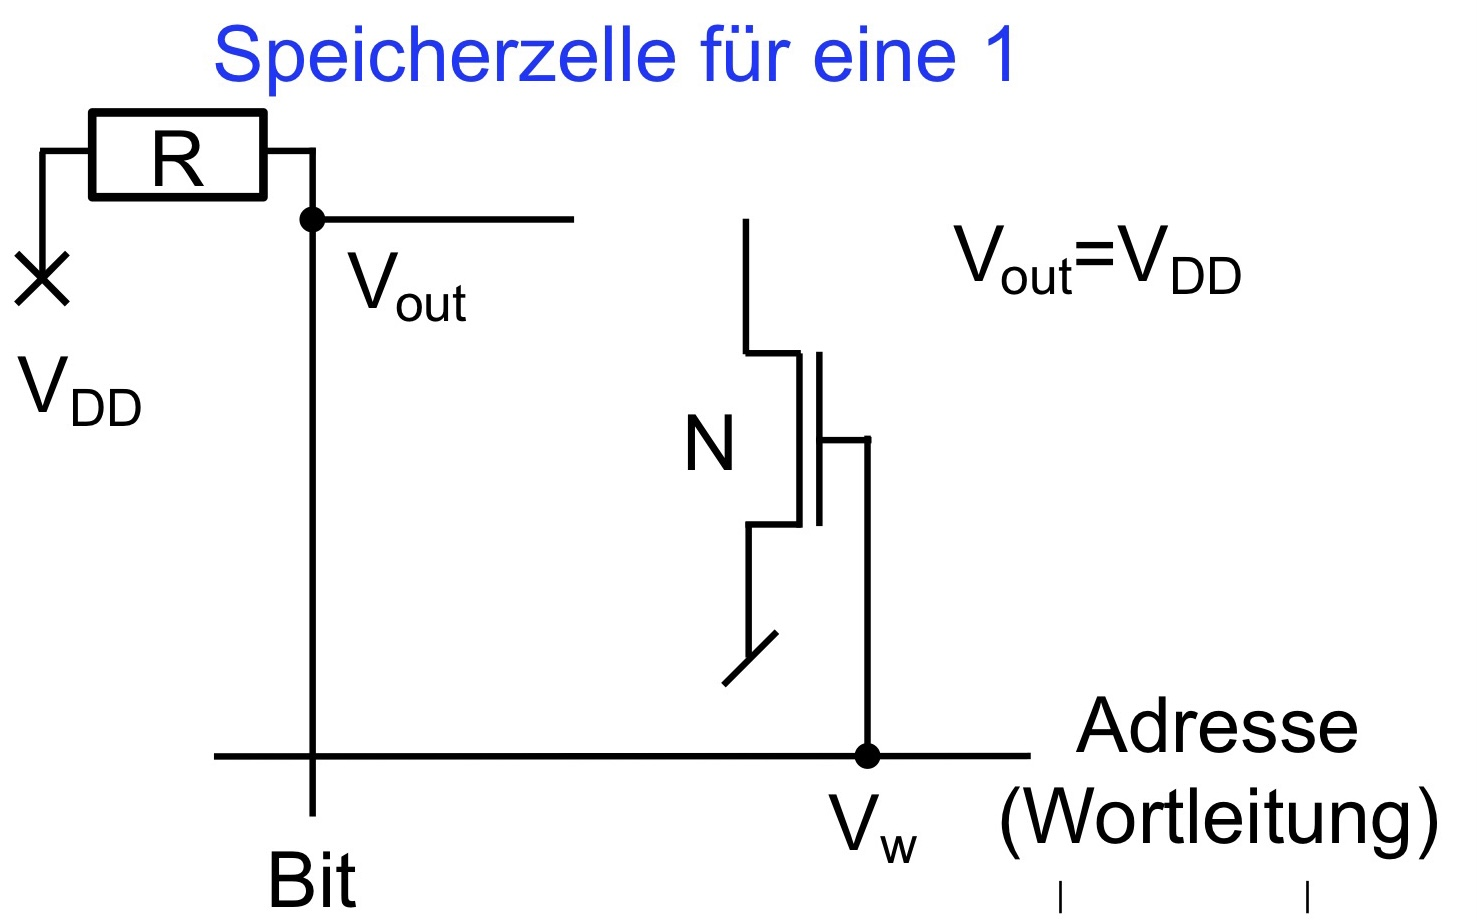
\includegraphics[width = 30mm]{images/rom_1.JPG}
    \end{minipage}
\end{center}